\section{Introducci�n}

\begin{frame}{OFDM}
  \begin{columns}[T]
    \begin{column}{.3\textwidth}
      \begin{itemize}
        \item Orthogonal Frequency Divider Multiplexing
        \item<2-> Divide la informaci�n en m�ltiples frecuencias
        \item<3-> Bandas de frecuencia solapadas
      \end{itemize}
    \end{column}
    
    \begin{column}{.7\textwidth}
      \uncover<2->{
        \alt<2>{
          \begin{center}
            \includegraphics[scale=0.17]{./figures/freq_mux.png}
          \end{center}
        }{
        %\uncover<4->{
          \begin{center}
            \includegraphics[scale=0.17]{./figures/freq_ort.png}
          \end{center}
        }
      }
    \end{column}
  \end{columns}
  
  \begin{itemize}
    \item<4-> Representaci�n matem�tica
  \end{itemize}
  \uncover<4->{
	  \begin{equation}
		s_{k}(t-kT) =
		%	\begin{cases}
			\sum\limits_{i=-N/2}^{N/2-1} x_{i,k} e^{j2\pi
			\left(\frac{i}{T}\right)(t-kT)}
		%	\end{cases}
		\end{equation}
	}
	
  \begin{itemize}
    \item<5-> Asumiendo que $x_{i,k}$ es constante a lo largo del per\'iodo de s\'imbolo $T$, se puede utilizar una IDFT\slash DFT para modular.
  \end{itemize}
  
%   \begin{columns}[T]
%     \begin{column}{.5\textwidth}
%       \uncover<6->{
%         \begin{center}
%           \advance\leftskip-0.2cm
%           \includegraphics[scale=0.26]{./figures/hard_mod.png}
%         \end{center}
%       }
%     \end{column}
%     
%     \begin{column}{.5\textwidth}
%       \uncover<8->{
%         \begin{center}
%           \advance\leftskip-0.2cm
%           \includegraphics[scale=0.26]{./figures/soft_mod.png}
%         \end{center}
%       }
%     \end{column}
%   \end{columns}
	
  
 
\end{frame}

\begin{frame}{FFT}
  \Fontit
  \begin{itemize}
    \item<1-> Transformada r�pida de Fourier
    \item<2-> Sumas, restas y multiplicaciones
    \item<3-> Cada salida = suma y resta de todas las entradas
  \end{itemize}

  \vfill

  \uncover<3->{
    \begin{center}
      \advance\leftskip-0.2cm
      \includegraphics[scale=0.30]{./figures/soft_mod.png}
    \end{center}
  }

\end{frame}
% 
% \begin{frame}{FPGA}
% 
% \begin{columns}[T]
%   \begin{column}{.2\textwidth}
%       \uncover<2->{
%         \alt<2>{
%         \begin{center}
%           \advance\leftskip-0.2cm
%           \includegraphics[scale=0.20]{./figures/circ_good.png}
%         \end{center}
%         }{
%         \begin{center}
%           \advance\leftskip-0.2cm
%           \includegraphics[scale=0.20]{./figures/circ_bad.png}
%         \end{center}
%         }
%       }
%     \end{column}
%     \begin{column}{.2\textwidth}
%       \uncover<4->{
%         \begin{center}
%           \advance\leftskip-0.2cm
%           \includegraphics[scale=0.13]{./figures/flecha.png}
%         \end{center}
%        }
%     \end{column}
%     
%     \begin{column}{.2\textwidth}
%       \uncover<5->{
%         \alt<5>{
%         \begin{center}
%           \advance\leftskip-0.2cm
%           \includegraphics[scale=0.20]{./figures/circ_good.png}
%         \end{center}
%         }{
%         \begin{center}
%           \advance\leftskip-0.2cm
%           \includegraphics[scale=0.20]{./figures/circ_bad.png}
%         \end{center}
%         }
%       }
%     \end{column}
%     \begin{column}{.2\textwidth}
%       \uncover<6->{
%         \begin{center}
%           \advance\leftskip-0.2cm
%           \includegraphics[scale=0.13]{./figures/flecha.png}
%         \end{center}
%        }
%     \end{column}
%     
%     \begin{column}{.2\textwidth}
%       \uncover<7->{
% %         \alt<7>{
%         \begin{center}
%           \advance\leftskip-0.2cm
%           \includegraphics[scale=0.20]{./figures/circ_good.png}
%         \end{center}
% %         }{
% %         \begin{center}
% %           \advance\leftskip-0.2cm
% %           \includegraphics[scale=0.20]{./figures/circ_tick.png}
% %         \end{center}
% %         }
%       }
%     \end{column}
%     
%     
%     
%   \end{columns}
%   
%   \vfill
%   
%   \uncover<8->{
% 	  \begin{center}
% 		  \advance\leftskip-0.2cm
% 		  \includegraphics[scale=0.26]{./figures/fpga_design.png}
% 	  \end{center}
%   }
% 
% \end{frame}
% 
% \begin{frame}
% 	\begin{center}
% 	\Huge MOTIVACIÓN Y OBJETIVOS
% 	\end{center}
% \end{frame}
% 
% \subsection{Motivacion}
% 
% \begin{frame}{Motivación}
%   \Fontit
%   \begin{itemize}
%     \item<1-> El avance de los sistemas de radio definidos por software
%     \item<2-> La flexibilidad que brindan las FPGAs para implementar sistemas complejos
%     \item<3-> La necesidad de sistemas de comunicaciones de código libre, eficientes y económicos
%     \item<4-> Aportar al desarrollo de un sistema de telecomunicaciones dentro del LSE
%     de la facultad
%   \end{itemize}
% \end{frame}
% 
\subsection{Objetivos}
\begin{frame}{Objetivos}
  \Fontit
  \begin{itemize}
    \item<1-> Dise�ar un modulador/demodulador OFDM para un sistema de telecomunicaciones definido por
    software que cumpla con el est�ndar ISDB-T
    \item<2-> Que sirva tambi�n como unidad de c�mputo FFT/IFFT para procesamiento de se�ales.
    \item<3-> Requerimientos
      \begin{itemize}
          \Fontitit
		  \item<4-> Longitud configurable, incluyendo al menos 2K, 4K y 8K muestras
		  (ISDB-T).
		  \item<5-> Frecuencia de muestreo m�nima de $8126984$ sps (seg�n est�ndar
		  ISDB-T)
		  \item<6-> Entrada y salida continua
		  \item<7-> Aritm�tica de punto fijo
		  \item<8-> Unidad de escalamiento configurable en ejecuci�n con opci�n de seleccionar la etapa a escalar y el m�todo (redondeo/truncamiento)
		  \item<9-> Bajo consumo de recursos comparados con otras
		  implementaciones\footnotemark \footnotemark
	  \end{itemize}
	\end{itemize}
	\uncover<9->{
	\footnotetext[1]{Implementaci�n abierta orientada a ISDB-T: Melo, R.,
	Salom\'on, F., Valinoti, B., (2016) ``IP core FFT configurable en Runtime''}
	\footnotetext[2]{Implementaci�n propietaria Xilinx LogiCORE FFT 7.1}}
\end{frame}

\begin{frame}{Objetivos}
  \Fontit
  \begin{itemize}
    \item<1-> Realizar una evaluaci�n de desempe�o
    \begin{itemize}
      \Fontitit
      \item<2-> Funcional
      \item<3-> Ruido / error
      \item<4-> Distorsi�n arm�nica
      \item<5-> Recursos de HW
    \end{itemize}
    \item<6-> Realizar una comparativa con desarrollos de terceros para evaluar el dise�o realizado
    \item<7-> Proponer trabajos futuros para continuar y mejorar el dise�o.
 \end{itemize}
\end{frame}
